\documentclass[a4paper,fleqn,12pt]{article}

%%%%%%%%%%%%%%%%%%%%


\usepackage[]{geometry}
\usepackage[latin1, utf8]{inputenc}
\usepackage[UKenglish]{babel}
\usepackage[UKenglish]{isodate}
\usepackage{amsmath}
\usepackage{amsfonts}
\usepackage{amssymb}
\usepackage{amsthm}
\usepackage{graphicx}
\usepackage{chngpage}
\usepackage{calc}
\PassOptionsToPackage{hyphens}{url}
\usepackage{hyperref}
\usepackage[nameinlink]{cleveref}
\usepackage{fancyhdr}
\usepackage{titletoc}
\usepackage[explicit]{titlesec}
\usepackage[square, numbers]{natbib}
\usepackage[dvipsnames]{xcolor}
\usepackage[sc]{mathpazo}
\linespread{1.05}
\usepackage[T1]{fontenc}
\usepackage[backgroundcolor=gray!5, hidealllines=true, roundcorner=10pt]{mdframed}
\usepackage{multirow}
\usepackage{subfig}
\usepackage{pgf-pie}
\hypersetup{
	colorlinks=true,
	linkcolor=black,
	urlcolor=black,
	citecolor=black
}
\usepackage[nomap]{FiraMono}
\usepackage{pdfpages}

\setlength{\parindent}{0mm}
\setlength{\parskip}{\medskipamount}
\renewcommand\baselinestretch{1.2}

\cleanlookdateon{}

\makeatletter
\newcommand{\@assignment}[0]{Assignment}
\newcommand{\assignment}[1]{\renewcommand{\@assignment}{#1}}
\newcommand{\@supervisor}[0]{}
\newcommand{\supervisor}[1]{\renewcommand{\@supervisor}{#1}}
\newcommand{\@yearofstudy}[0]{}
\newcommand{\yearofstudy}[1]{\renewcommand{\@yearofstudy}{#1}}
\newcommand{\txt}[1]{\mintinline{text}{#1}}
\newcommand{\scala}[1]{\mintinline{scala}{#1}}
\makeatletter

\newtoggle{IsDissertation}


%%%%%%%%%%%%%%%%%%%%%%%%%%%%%%%%%%%%%%%%%%%%%%%%%%%%%%%%%%%%%%%%%%%%%%%%%%%%%%%
%% Project-specific configuration
%%%%%%%%%%%%%%%%%%%%%%%%%%%%%%%%%%%%%%%%%%%%%%%%%%%%%%%%%%%%%%%%%%%%%%%%%%%%%%%

\author{Your name}
\title{Project title}
% \supervisor{Your supervisor's name}
% \yearofstudy{3\textsuperscript{rd}}

%%%%%%%%%%%%%%%%%%%%%%%%%%%%%%%%%%%%%%%%%%%%%%%%%%%%%%%%%%%%%%%%%%%%%%%%%%%%%%%


\assignment{Project specification}

%%%%%%%%%%%%%%%%%%%%

\pagestyle{plain}
\renewcommand{\headrulewidth}{0.0pt}

\makeatletter
\fancypagestyle{plain}{
	\fancyhf{}
    \fancyfoot[C]{\thepage}
}
\makeatother

%%%%%%%%%%%%%%%%%%%%
\begin{document}

\makeatletter
\begin{titlepage}

    % do not show the assignment name for the dissertation
    \iftoggle{IsDissertation}
    {
        \textbf{\Huge \@title} \\[1.5cm]
    }
    {
        \textbf{\Huge \@title} \\
        \Large \@assignment \\[1.5cm]
    }
    \Large \textbf{\@author} \\
    Department of Computer Science \\
    University of Warwick \\

    % include the supervisor and year of study if the are specified and its the disseration
    \iftoggle{IsDissertation}{
        \ifdefempty{\@supervisor}{}{
            Supervised by \@supervisor \\
        }\ifdefempty{\@yearofstudy}{}{
            Year of Study: \@yearofstudy \\
        }
    }{}

    \vfill

    % include the current date for the dissertation
    \iftoggle{IsDissertation}{\today}{}

    \begin{adjustwidth}{-\oddsidemargin-1in}{-\rightmargin}
        \centering
        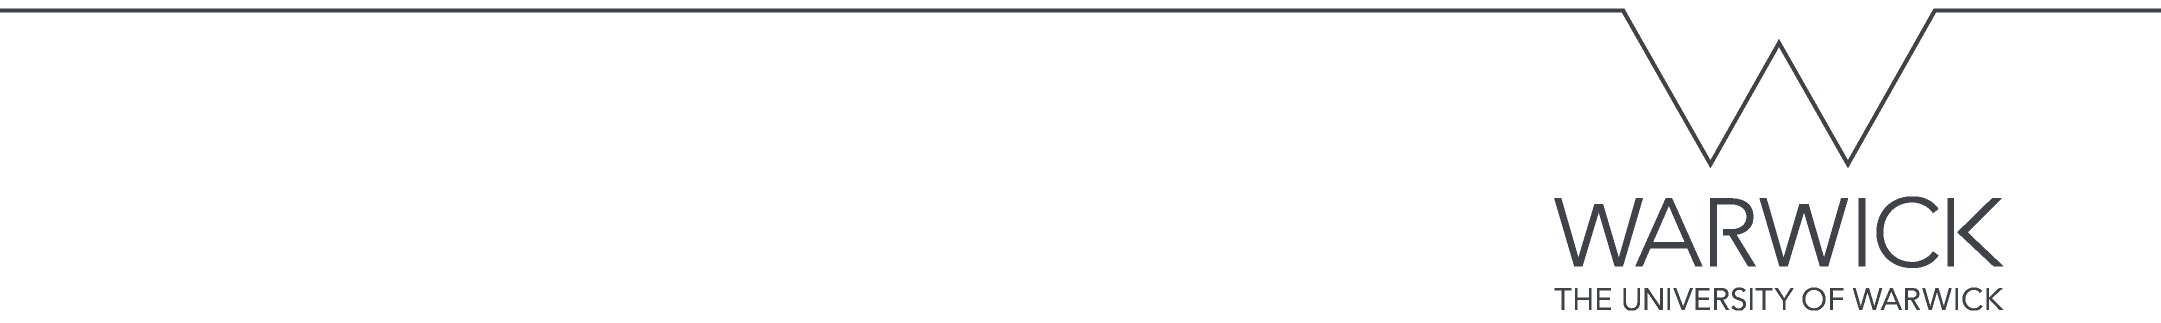
\includegraphics[width=\paperwidth]{../common/line.png}
    \end{adjustwidth}

    \vspace*{-3.5cm}

\end{titlepage}
\makeatother


\pagestyle{plain}

\section{Introduction}
Traditionally, general-purpose microcontrollers necessitate the inclusion of a wide variety of hardware interfaces such as UART, SPI, and I2C to interface with a broad range of peripherals. Each of these interfaces has different hardware requirements, and is costly in development time, chip area, and system power. These interfaces are often emulated using software techniques known as "bit-banging", but such techniques are usually inefficient and have poor performance.

The aim of this project is to develop state machine-based programmable I/O blocks which are able to emulate any hardware interface or implement any communication protocol, via programming using a small assembly-like DSL. These blocks will then be integrated with open-source RISC-V cores to create a flexible and compact microcontroller, ideal for use in low power, low cost embedded applications. This microcontroller would be applicable for any use in which traditional hardware interfaces are needed, but also for applications which have specific or highly custom I/O requirements, without the need for programmable logic (as is found in FPGAs) or custom hardware.

\section{Background}

The primary purpose of embedded systems and microcontrollers is usually to interact with the real world via sensors, actuators, LEDs, speakers, etc, but communicating with such hardware can be difficult due to the need for high frequencies and precise timing requirements. Computers and microcontrollers include dedicated hardware for high-speed interfaces: SATA and PCIe are common in desktop-class hardware and used to interface with consumer hardware, but interfaces such as UART, SPI, I2C, PWM and I2S are more general-purpose buses usually found in microcontrollers and designed for use with a wide variety of electronics devices. These protocols are also simpler and cheaper (in terms of power, space and money) to implement than the likes of SATA, making them ideal for lower-cost devices such as the RP2040. All of these interfaces have different hardware and software requirements, and the cost and complexity associated with implementing all of these in a device may mean you end up with lots of interfaces you don't need, or not enough of a single type of interface.

A common alternative to using dedicated hardware is to use the CPU to control the GPIO (General Purpose I/O) pins, implementing the control and timing processes in software: a process known as 'bit-banging'. However, general-purpose software processors are generally not designed to do this, and maintaining precise timing requirements at high speed is very hard, especially when the processor has other work to do. For example, SPI can run at speeds of up to 100MHz,

The usual solution to custom interface requirements is FPGAs: programmable hardware devices that allow a designer to implement whatever hardware they wish. These are very flexible but come at a high price, and there is also the need to implement some other software processor. 'Soft' CPU cores can be implemented in FPGAs, and some embedded systems such as the Xilinx Zynq SoCs combine traditional processing cores with programmable logic slices, connected over the system bus as shown in figure 3. FPGAs also present a very different programming model, as programmers are not writing software but designing hardware \citep{picosdk}.

\section{Objectives}
\section{Timeline}
\section{Methodology}
\section{Resources}
\section{Risk Assessment}
\section{Legal, Social and Professional Issues}
\bibliographystyle{../common/plainnat}
\bibliography{../common/bibliography}

\end{document}
